\section{\texttt{React}}

On the last day of the third week, we started discussing \texttt{React}, a user interface library created by Facebook on \texttt{JavaScript}. I had almost no experience with both \texttt{React} and \texttt{JavaScript}. 

\subsection{MPA and SPA}

% MPA and SPA
We started the discussion with MPA (multiple page applications) and SPA (single page applications) and why SPA should be chosen over MPA. \texttt{React} helps developers to develop SPA by using JavaScript and virtual DOM. Since our primary concern will have been learning \texttt{React}, we talked about its advantages and limitations and compared \texttt{React} with other frameworks and libraries by looking at the trends to have a better perspective.

% Rendering UI
We started with the \texttt{React} elements and continued with how we could render them. After learning the basics, we talked about JSX, a syntax extension to JavaScript that allows \texttt{React} elements to be written inside JavaScript using HTML tags. Since JSX has many different features, such as styling the elements and inserting JavaScript variables, we had to spend much time on it solving mini coding challenges.

\subsection{Functional and Class Components}

% Functional components and class components
\begin{wrapfigure}{r}{0.3\textwidth}
  \centering
  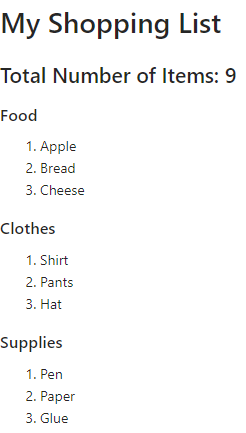
\includegraphics[width=0.3\textwidth]{img/shopping-app.png}
  \caption{Basic Shopping List App}
\end{wrapfigure}
We moved into components. A \texttt{React} component can be defined as an independent, reusable component that outputs the \texttt{React} element. We compared the class and functional components and discussed their usage differences. I realized that I tended to use class components because of the OOP and class familiarities, although functional components are excessively used in the sector.

After these, we solved an example, which can be called Shopping List App. It was a simple shopping list without adding or removing options, but it only showed the provided list. After we coded the exercise, our mentor also coded the exercise to show us another perspective.

\subsection{States}

% States
Then we discussed a crucial topic and feature of \texttt{React}: \texttt{States}. We talked about what a state is and how it is used. We then jumped into another critical issue in states: setting/updating the state. We realized and learned how to fix the different behaviors of setting states.

\subsection{Life Cycle Methods}

% Life Cycle Methods
Another essential topic was the life cycle methods of class components. While rendering and mounting the component, \texttt{React} runs various methods on the components at multiple phases. Life cycle methods can be used for specific purposes according to phases.

\subsection{Event Handlers}

% Event Handlers
Event handling is pretty similar to HTML events. We discussed that we could achieve some effects by using event handlers. For example, sending a request when a button is clicked or changing the state of a variable when a key is pressed can be achieved by event handlers.

\subsection{Promises, Back-end Requests, and JWT}

% Promises and Back-end Request
After the basics and some advanced topics, we moved into the back-end requests. Before talking about them, we discussed the promises, a feature of JavaScript. For back-end requests, we conversed about Axios. Axios provides support to different request types and configs and is easy to use.

% JWT
We briefly discussed JWT tokens used for token-based authentication instead of password authentication every time.
